%Préambule du document :
\documentclass[12pt, a4paper]{book}
%\usepackage[latin1]{inputenc} 
\usepackage[utf8]{inputenc} % accents
\usepackage{gensymb} % degree symbol ° (\degree)
\usepackage[T1]{fontenc} % | "`pipe"' character
\usepackage{graphicx}
\usepackage{titling}
\usepackage{amssymb} 
\usepackage{minitoc} % chapter's tocs
\usepackage{authblk} % author affiliations
\usepackage{fancyhdr} % modify the headers
\usepackage{tabularx} % tables not larger than A4
\usepackage[table]{xcolor} %colors inside the tables
\usepackage{float}
\usepackage{multicol} % multiple columns in some sections
\usepackage[inner=2cm,outer=2cm]{geometry} %A4 margins
\usepackage{siunitx}
\usepackage[labelfont=bf, margin=0.5cm]{caption} % for figure captions in minipages
\usepackage{hyperref} %link references (toc, citations) inside document
\usepackage{natbib} % to cite with parentheses and plain text et only year if you please...
\usepackage{amsmath}
 \usepackage{fixltx2e} % allows overrightarrow to be in caption
 \MakeRobust{\overrightarrow}




\bibliographystyle{plainnat} % reference style
\renewcommand{\bibname}{References} %Rename "`bibliography"' => "`references"'

\hypersetup{
    colorlinks,
    citecolor=brown,
    filecolor=green,
    linkcolor=red,
    urlcolor=blue
}
\hypersetup{linktocpage}


\pagestyle{fancy}
\fancyhead{}
\fancyfoot{}
\fancyhead[RO,LE]{\thepage}
\fancyhead[LO]{\leftmark}
\fancyhead[RE]{\rightmark}
\setcounter{tocdepth}{1} % we only want chapters and sections in toc
\setcounter{minitocdepth}{2} %we want sections and subsections in chapters' minitocs

\pretitle{%
  \begin{center}
  
  
\includegraphics[width=17cm]{../Logo_software.png}\\[\bigskipamount]
}
\posttitle{
\\
  \includegraphics[width=5.8cm]{tutorial07.png}\\[\bigskipamount]
\end{center}}

%\postdate{
%
\includegraphics[width=15cm]{logo_affiliations.png}
%}

\title{Tutorial 07: thickness within objects and scalar normalization}



%\titlepicture[width=13cm]{Logo_software.png}
\author{Renaud LEBRUN}
\affil{Institut des Sciences de l'Evolution, Université de Montpellier, France}
\date{\today} 

\def\chaptername{Tutorial}
\setcounter{chapter}{7}
%Corps du document :
\begin{document}

	\dominitoc

\maketitle


\faketableofcontents

%\chapter{Working with landmarks}
\addstarredchapter{Thickness within objects and scalar normalization}

\markboth{Tutorial 07: thickness within objects and scalar normalization}{}

\minitoc 
Tutorial 07 includes:
\begin{itemize}
\item One .ntw (MorphoDig project) file
\item Two .vtk surface files representing right femurs of \textit{Erythrocebus patas} and \textit{Papio} sp.
\item Two .pos (position) files 
\item One .tgp (tag map) file 
\item One .txt file containing the summary of the Normalized thickness scalar array for the two femurs.
\item The present .pdf document
\end{itemize}



\section{About the specimen}

%\addcontentsline{toc}{section}{About the specimen}
The surface files enclosed in this tutorial represent three-dimensional reconstruction of the right femurs of two primates, \textit{Erythrocebus patas} and \textit{Papio} sp. from the collections of the Institut des Sciences de l'Evolution de Montpellier (ISEM), Université de Montpellier. The 3D data were obtained by computerized microtomography at the MRI \si{\micro}CT platform housed at the ISEM.
Before using this tutorial, please download and read MorphoDig User Guide. \\

Download and unzip the files associated to this tutorial. Open MorphoDig.


\section{A brief overview of enclosed files}
The present tutorial contains a project .ntw file, which is useful to open the two femurs
 in convenient positions. Open the enclosed .ntw file (File->Open Project, then select
"Primate\_femur\_thickness.ntw"). Once loaded, the two femurs are opened, are given the positions
enclosed in the two position files, and a color. Note that the newly opened surfaces are unselected.


\section{Tutorial}

\subsection{Thickness within objects}
Each femur 3D representation already contains a "Thickness" scalar array. This thickness was produced as follows (see also Fig. \ref{compute_thickness}, p.\pageref{compute_thickness}): \\
1) The femur of \textit{Erythrocebus patas} was selected \textbf{alone} (the femur of \textit{Papio} sp. should remain unselected), and the "Compute thickness within selected objects" dialog was opened (Scalars->Compute thickness within each selected surface). \\
2) The Maximal thickness was set to "3mm", as we do not expect bone thickness to exceed 3mm within this bone. Note that in order to minimize computation time, this value should be set as low as possible. We could have chosen a larger value, which would lead to the same result but would take a significantly larger amount of time.\\
3) The femur of \textit{Erythrocebus patas} was unselected. Then the femur of \textit{Papio} sp. was selected \textbf{alone} and the "Compute thickness within selected objects" dialog was opened once again. \\
4) The Maximal thickness was set to "12mm", as we do not expect bone thickness to exceed 12mm within the femur of \textit{Papio} sp. Note that this value was once again set as low as possible in order to minimize computational time.\\

\begin{figure}
  \centering
  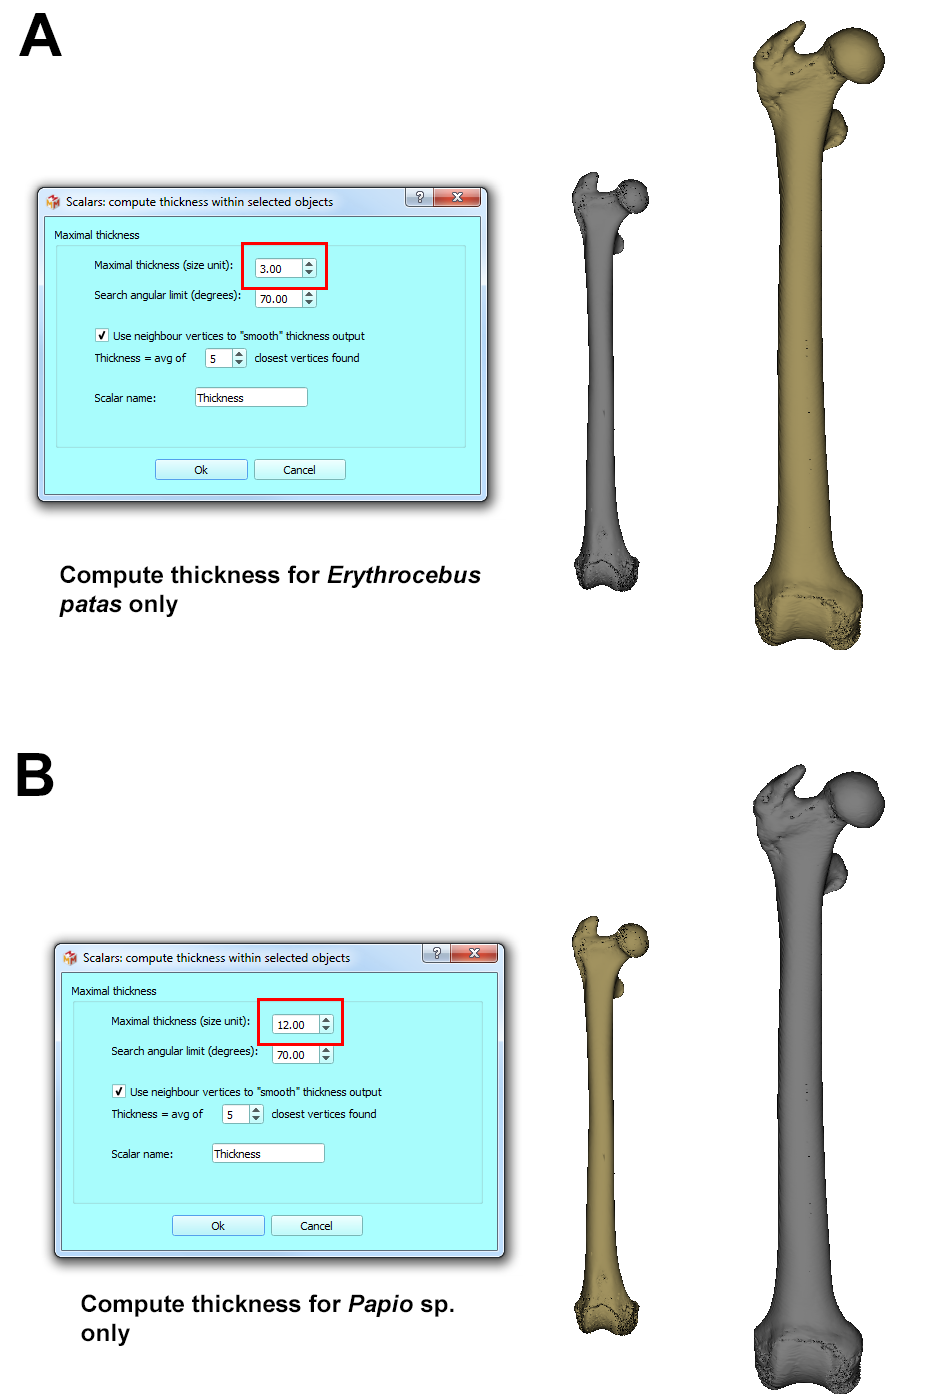
\includegraphics[scale=0.45]{Compute_thickness.png}
\caption{Bone thickness computation. \textbf{A:} The femur of \textit{Erythrocebus patas} (left) was selected \textbf{alone}, and the maximal thickness value to be looked for was set to "3mm". \textbf{B:} The femur of \textit{Papio} sp. (right) was selected \textbf{alone}, and the maximal thickness value to be looked for was set to "12mm".}	
\label{compute_thickness}
 \end{figure}

Baboons (\textit{Papio}) are much larger primates than patas monkeys (\textit{Erythrocebus patas}). As a consequence we expect than baboon's femurs, as a general rule, are much thicker than patas' femurs for all regions of that bone, and that bone thickness distribution of baboons and patas monkeys are not directly comparable. The difference between bone thickness between a baboon and a patas monkey is illustrated in Fig. \ref{thickness}, p.\pageref{thickness}. 

\begin{figure}
  \centering
  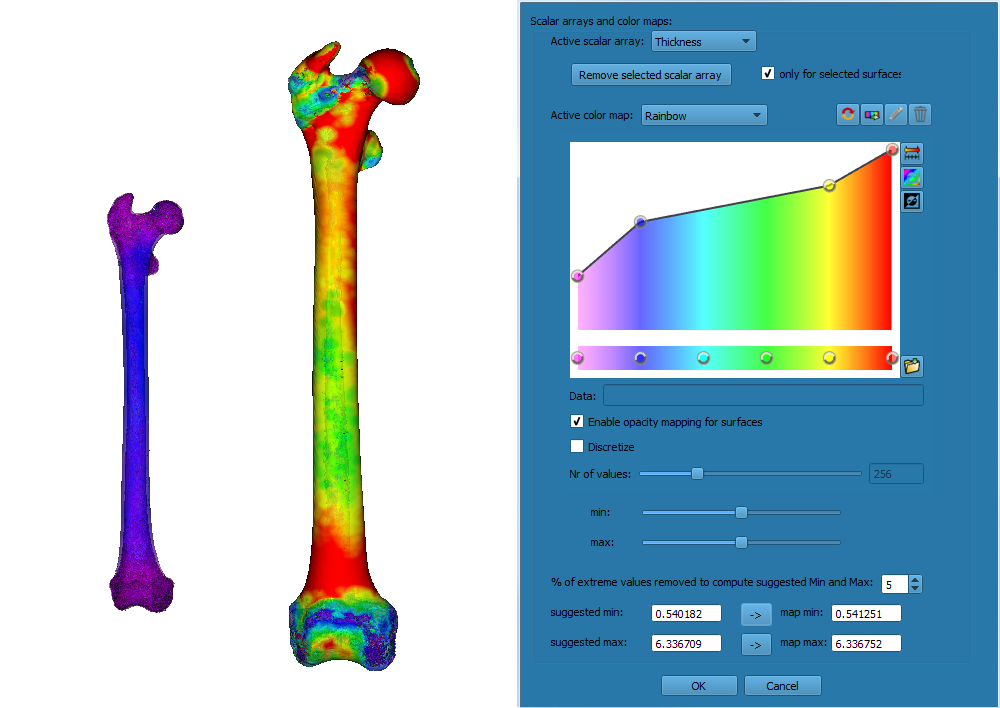
\includegraphics[scale=0.45]{Thickness.png}
\caption{Thickness distribution differences between \textit{Erythrocebus patas} and \textit{Papio} sp. The color map was set to range between around 0.5mm and 6.3mm. The femur of \textit{Erythrocebus patas} (left) is much thinner than that of \textit{Papio} sp. (right) for all region, which makes a direct comparison of bone distribution patterns difficult between those two specimens.}	
\label{thickness}
 \end{figure}

\subsection{Scalar normalization.}
In order to be able to compare bone thickness distribution patterns between specimens of different body size and body mass, allometry has to bee taken into account  (that is: differences in bone thickness for which size and body mass differences are responsible). A possible solution is to normalize bone thickness scalar array within each specimen. 
Each femur 3D representation already contains a "Norm\_thickness" scalar array. This array was produced as follows (see also Fig. \ref{normalize_thickness}, p.\pageref{normalize_thickness}): \\
1) Select "Thickness" to be the active scalar array.\\
2) The femur of \textit{Erythrocebus patas} (left) was selected \textbf{alone} (the femur of \textit{Papio} sp. (right) should remain unselected), and the "Scalars: normalization" dialog was opened (Scalars->Normalize or rescale active scalars for each selected surface). \\
3) In order to minimize the influence of the most extreme values, 5\% of the minimal and maximal values were removed.\\
4) The active scalar was set as "Thickness" again. \\
5) The femur of \textit{Erythrocebus patas} (left) was unselected. Then the femur of \textit{Papio} sp. (right) was selected \textbf{alone} and the "Scalars: normalization" dialog was opened once again. \\
6) Again, in order to minimize the influence of the most extreme values, 5\% of the minimal and maximal values were removed.\\



\begin{figure}
  \centering
  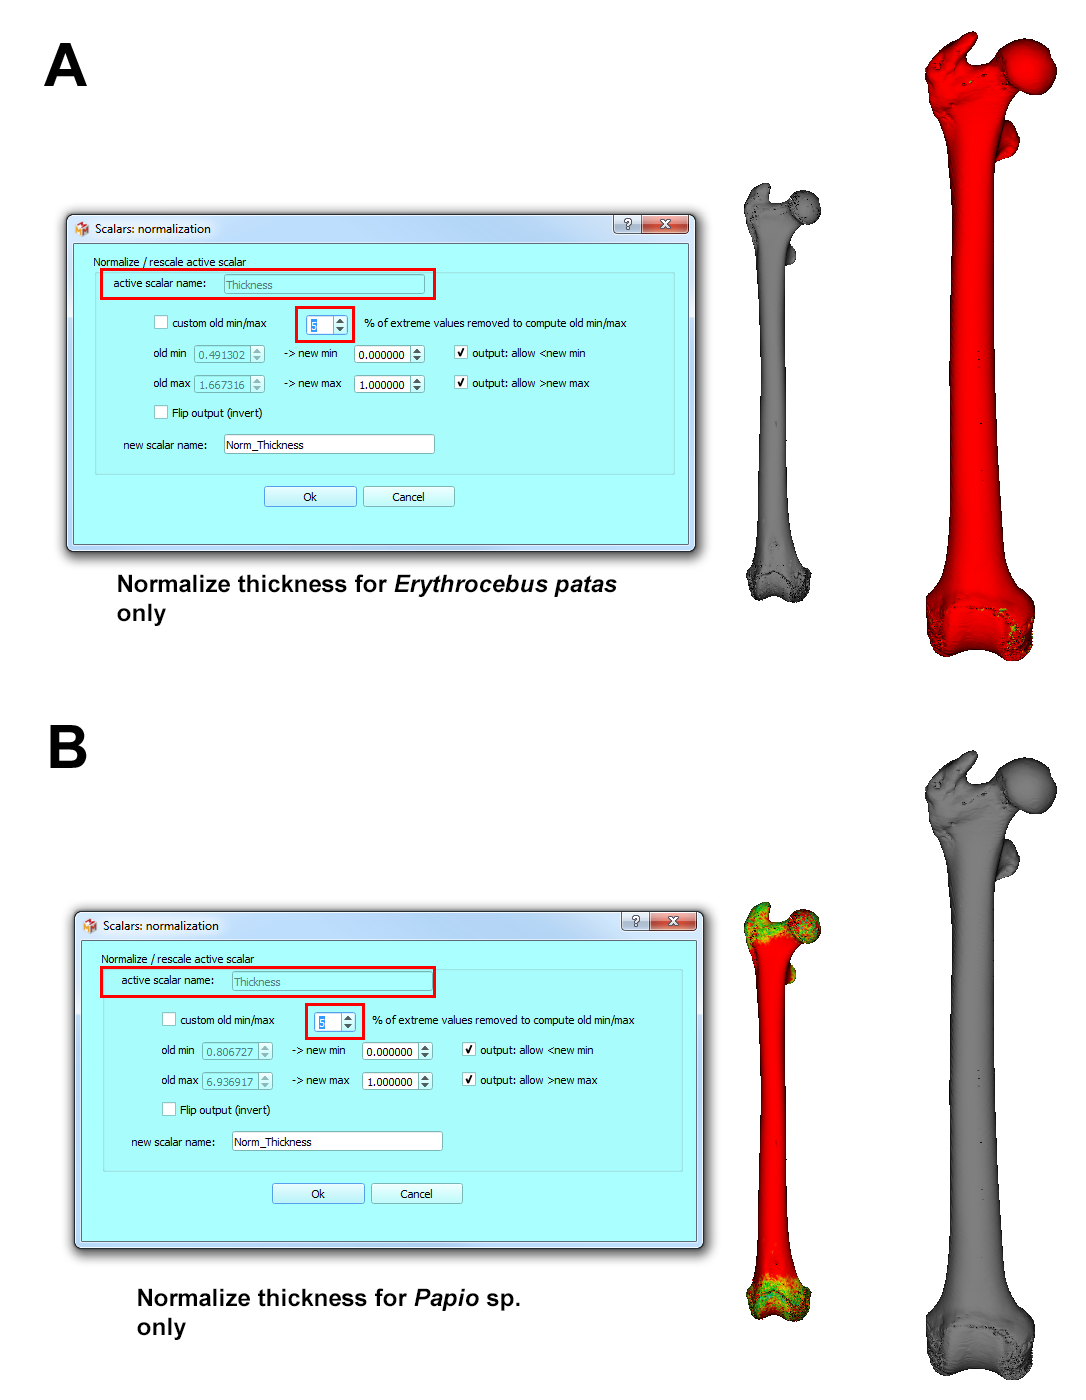
\includegraphics[scale=0.43]{Normalize_thickness.png}
\caption{Thickness array normalization. \textbf{A:} The active scalar is "Thickness." The femur of \textit{Erythrocebus patas} (left) was selected \textbf{alone}, and 5\% of the most extreme maximal and minimal values were excluded from the normalization process. \textbf{B:} The femur of \textit{Papio} sp. (right) was selected \textbf{alone}, and 5\% of the most extreme maximal and minimal values were excluded from the normalization process.}	
\label{normalize_thickness}
 \end{figure}

Thickness distribution patters of the right femurs of (\textit{Papio}) sp. and (\textit{Erythrocebus patas}) are now much easier to compare and describe (Fig. \ref{normthickness}, p.\pageref{normthickness}). 

\begin{figure}
  \centering
  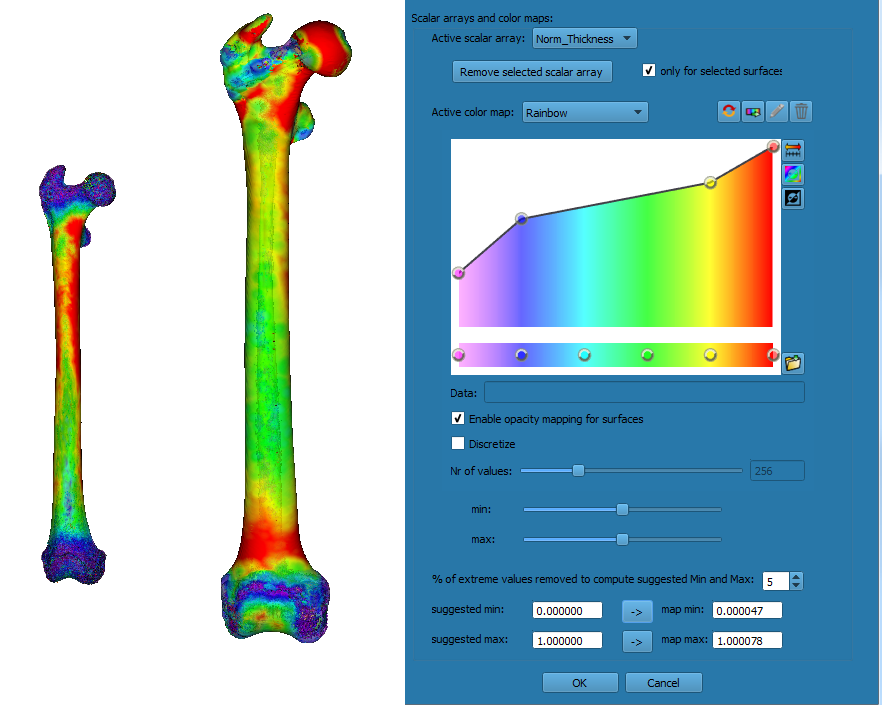
\includegraphics[scale=0.45]{NormThickness.png}
\caption{Normalized thickness distribution in \textit{Erythrocebus patas} and \textit{Papio} sp. The color map was set to range between around 0 and 1 (no unit). Normalization makes it possible to compare directly thickness distribution patterns between these specimens. For instance, the femur of \textit{Erythrocebus patas} (left) and express a relatively lower thickness in the proximal epiphysis  region (top) than  that of \textit{Papio} sp. (right), while the distal epiphyses are much more similar. The shafts of these two femurs also express differences: for \textit{Erythrocebus patas}, the relatively thickest shaft region is located proximally (top), while the relatively thickest shaft region of \textbf{Papio} sp. is situated distally (bottom). }	
\label{normthickness}
 \end{figure}

\subsection{Using tags to compute scalar infos (mean, variance etc.) within different regions}
At this point you may save information (mean, median, variance, 5\% and 95\% quantiles etc.) for the currently computed scalars (Thickness and "Norm\_Thickness") for these two bones. To do so, select the desired active scalar array, and click on "File->Measurements->Save active scalars infos (mean, median, variance ...) of selected surfaces". \\

You might also be interested to compute mean bone thickness, variance etc. for different regions of these femurs, such as the shaft, the proximal epiphysis and the distal epiphysis. To do so, you have to use tag arrays.\\

A tag array named "Tags" is enclosed within the two .vtk surface files. To display those tags, the array display mode button must be pressed (
\includegraphics[scale=0.7]{../images/04/show_color_scale.png}), and the "\textbf{Tags}" array must be selected as the currently active array (
\includegraphics[scale=0.5]{scalarcombo_tag.png}), see  Fig. \ref{tags}, top, p.\pageref{tags}. The way tag arrays are translated into colors is set up using a tag map, also referred to as a "Lookup table" (LUT) or color transfer function. Such a LUT is enclosed within the tag map file ("Primate\_femur\_thickness.tgp"), which was opened when loading the project.  Open the tags window ("File->Tags->Open Tags window", or click on "
\includegraphics[scale=0.7]{../images/04/tag_edit.png}". The Tag window should open (see Fig. \ref{tags}, bottom, p.\pageref{tags}), and should contain the tag names and associated colors defined in "Primate\_femur\_thickness.tgp". These three regions were tagged using the rubber band "
\includegraphics[scale=0.7]{../images/12/rubber_band.png}" tag tool. See MorphoDig user guide for further explanation regarding the Tags window and Tag edition with MorphoDig and also the tutorials dealing with tags.\\

\begin{figure}
  \centering
  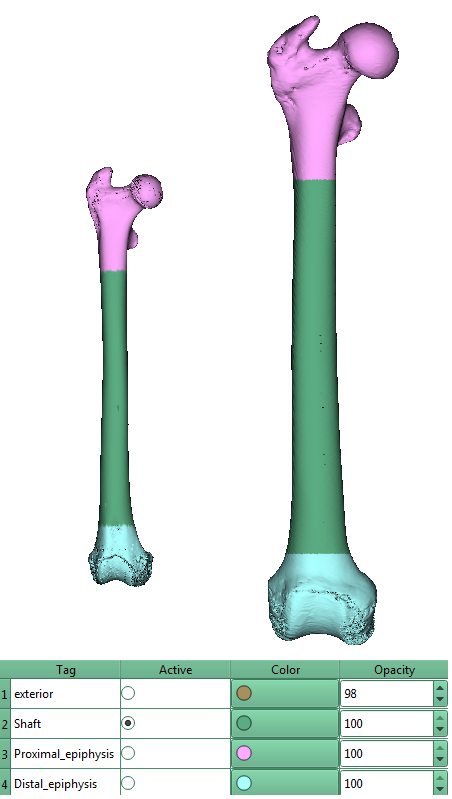
\includegraphics[scale=0.5]{Tags.png}
\caption{Tag array. \textbf{Top:} 3D rendering of the two primate femurs when the active array is "Tags". \textbf{Bottom:} corresponding color map. }	
\label{tags}
 \end{figure}

In order to compute bone thickness mean, median, variance, 5\% and 95\% quantiles etc. for the femur shaft, proximal epiphysis and distal epiphysis, select the two femurs and click on "File->Measurements->Save active scalars infos (mean, median, variance ...) of selected surfaces". Then make sure that the checkbox "Include scalar infos for each Tagged region" is checked, and taht the "Tags" array is selected  (Fig. \ref{scalars_infos} p.\pageref{scalars_infos}). The produced text file will contain also one line for each bone region of each bone.
\begin{figure}
  \centering
  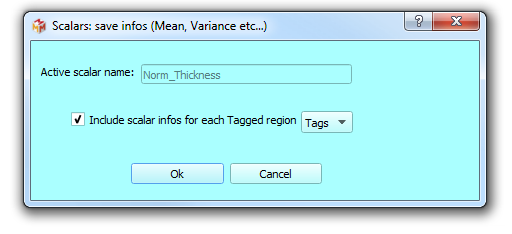
\includegraphics[scale=0.5]{Save_scalar_infos.png}
\caption{Save active scalars infos dialog. Note that the checkbox "Include scalar infos for each Tagged region" is checked, and the "Tags" array is selected.}	
\label{scalars_infos}
 \end{figure}
\section{Acknowledgements}
Thanks to the MRI imaging platform for the access to imaging facilities.

%\nocite{*}   % All bibliography items appear without citation in the text

%\cleardoublepage
%\phantomsection


%\addcontentsline{toc}{section}{References}

 %\bibliography{References}		
\end{document} 

